\documentclass[a4paper]{article}
 
\usepackage{amsmath}
\usepackage{graphicx}
\usepackage{caption}
\usepackage{subfigure}
\usepackage{epstopdf}
\usepackage[ansinew]{inputenc}
\usepackage{listings}
\usepackage{xcolor}
%\setlength{\oddsidemargin}{0cm}
%\setlength{\evensidemargin}{0cm}
%\setlength{\topmargin}{0cm}

\usepackage[]{algorithm2e}

\usepackage{a4wide}

\title{ Creating point neuron circuit from Allen mouse brain injection experiments }
%\author{Till Schumann}
%\date{}

\begin{document}
   \maketitle
   
   \section{Description}
   
   Allen Institute for Brain Science provides a high-resolution map of neural connections in the mouse brain.
   It contains several injection experiments. The provided datasets of the experiments 
   contain a 3D image of the injection and a 3D image of its axonal projection labeled by viral
   tracers. Based on this data the long range connections for the point neuron circuit of the mouse brain are generated.
   Therefore a set of experiments is used to connect neurons located at the injections
   to the neurons at the projections. Unfortunately all injections from these experiments do not
   cover the whole brain. So there are neurons which are not injected
   by any experiment. To overcome this limitation, we decided to use information from the nearest
   available injection whenever data was not available.
   Therefore all neurons which are not injected should use the projection
   from the nearest injection.
   
   \begin{figure}[ht!]
   	\begin{center}
        \subfigure[Injection sites - showing all available experiments]{%
            \label{fig:allInjections}
            \includegraphics[width=0.4\textwidth]{../connectionBrowser_allinjections.png}
        }
        \subfigure[Projection of one experiment]{%
            \label{fig:oneProjection}
            \includegraphics[width=0.32\textwidth]{../connectionBrowser_oneinjections.png}
       }
    	   \end{center}
    	\caption{%
        The pictures are inverted and copied from the Allen Brain Atlas.
     }%
   \label{fig:atlas}
   \end{figure}
   
   \begin{figure}[ht!]
   	\begin{center}
        \subfigure[Number of excitatory neurons per voxel]{%
            \label{fig:allInjections}
            \includegraphics[width=0.4\textwidth]{../exNeurons_numPerVoxel.png}
        }
        \subfigure[Neurons for which there are injections available (green) ]{%
            \label{fig:oneProjection}
            \includegraphics[width=0.35\textwidth]{../missing_experiments.png}
       }
    	   \end{center}
    	\caption{%
        The plots (x vertical and z horizontal axis) show a slice (along the y axis) of the 3D datasets. 
     }%
   \label{fig:atlas}
   \end{figure}
   \newpage
	\section{Implementation}
	To map pixels of the 3D pictures to neurons, the neurons are assigned to voxels, which represent the pixels.
	In a first step the best experiment is chosen for each voxel. The best experiment is specified as the experiment which
	injects the voxel and has the smallest total injection.
	Only the right hemisphere is considered. Experiments which have injections
	in the left hemisphere are mirrored along the z-axis. Thus we use a complete symmetric approach.
	In the second step all voxels in the right hemisphere, which have not received an experiment take the experiment
	from the nearest voxel, which has an experiment. Therefore for each not injected voxel a linear search iterates over its neighborhood
	with increasing distance. It picks the first match.
	In the third step the selected experiments are used to create connections from the neurons in the injected voxels to the neurons in the 
	projected voxels. A linear acceptance rejection method is used with a fixed degree of outgoing synapses for each neuron in the injected voxels.
	
    \begin{figure}[ht!]
   	\begin{center}
        \subfigure[Illustration injection per voxel]{%
            \label{fig:allInjections}
            
\includegraphics[width=0.15\textwidth]{cg_illustration_injection.eps}
        }
        \hspace{0.5cm}
        \subfigure[Illustration projection per voxel]{%
            \label{fig:oneProjection}
            
\includegraphics[width=0.15\textwidth]{cg_illustration_projection.eps}
       }
       \hspace{0.5cm}
       \subfigure[Remove injected area from projection area]{%
            \label{fig:allInjections}
            
\includegraphics[width=0.15\textwidth]{cg_illustration_merge.eps}
        }
        \hspace{0.5cm}
        \subfigure[Assign source and target neurons for generated connection]{%
            \label{fig:oneProjection}
            
\includegraphics[width=0.15\textwidth]{cg_illustration_neurons.eps}
       }
    \end{center}
    	\caption{%
        Assign injections and projections of experiments to neurons.
     }%
   \label{fig:atlas}
   \end{figure}	
	
	\begin{figure}[ht!]
   	\begin{center}
   		\subfigure[x-y slice]{%
            \label{fig:xy70}
            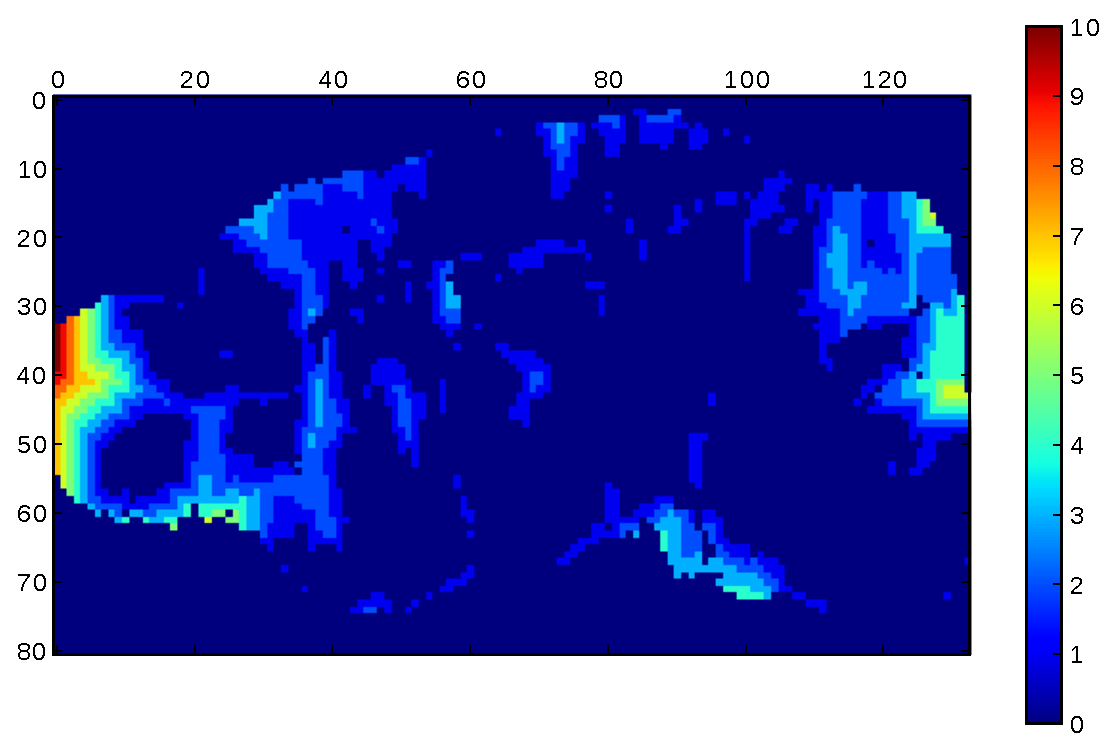
\includegraphics[width=0.45\textwidth]{distance_x_y_70.eps}
       }
        \subfigure[y-z slice]{%
            \label{fig:68yz}
            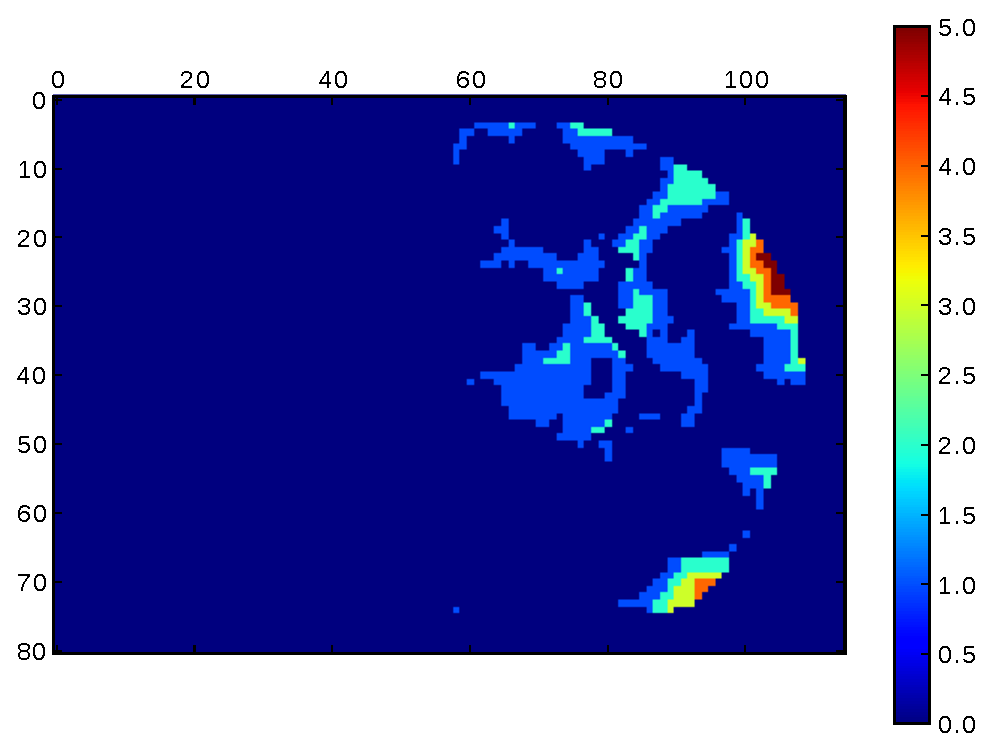
\includegraphics[width=0.4\textwidth]{distance_68_y_z.eps}
        }
        \subfigure[z-x slice]{%
            \label{fig:x40z}
            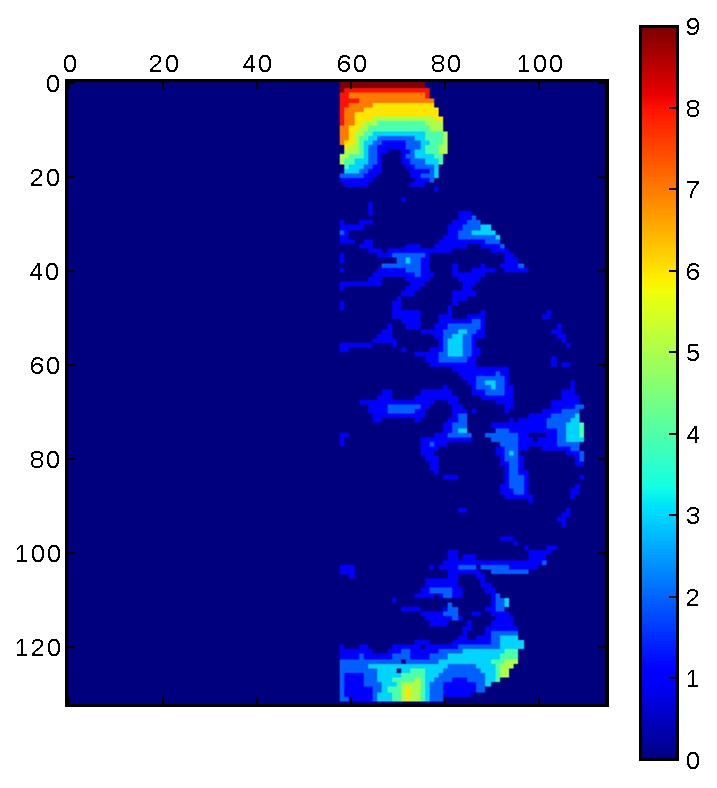
\includegraphics[width=0.4\textwidth]{distance_x_40_z.eps}
       }
    	   \end{center}
    	\caption{%
        For each voxel of the right hemisphere the figures show the distances to nearest injection. 
     }%
   \label{fig:distance}
   \end{figure}


\end{document}
